\documentclass[aps,pra,superscriptaddress,twocolumn]{revtex4-1}

\usepackage{graphicx}
\usepackage{amsmath}
\usepackage{amssymb}
\usepackage{hyperref}
\usepackage[utf8]{inputenc}
\usepackage{mathtools}
\usepackage[english]{babel}
\usepackage{bbm}
\hypersetup{colorlinks=true, linkcolor=blue, citecolor=blue, urlcolor=blue}
\usepackage{xcolor}
\usepackage{braket}

%===Newcommands============================
\DeclareMathOperator{\sgn}{sgn}
\newcommand{\ie}{i.\,e.,\ }
\newcommand{\Ie}{I.\,e.\,,\ }
\newcommand{\eg}{e.\,g.,\ }
\newcommand{\Eg}{E.\,g.\,,\ }
\newcommand{\cf}{cf.\ }
%
\newcommand{\re}{\mathrm{Re}}
\newcommand{\im}{\mathrm{Im}}
\newcommand{\abs}[1]{|#1|}
\newcommand{\ii}{\mathrm{i}}
\newcommand{\ee}{\mathrm{e}}
\newcommand{\proj}[1]{|#1\rangle\langle #1|}
\newcommand{\Tr}{\operatorname{Tr}}
\newcommand{\rr}{\mathbf{r}}
\newcommand{\pp}{\mathbf{p}}
\newcommand{\kk}{\mathbf{k}}
%
\newcommand{\cc}{\text{c.c.}}
\newcommand{\fref}[1]{\text{Fig.}~\ref{#1}}
\newcommand{\ffref}[1]{\text{Figs.}~\ref{#1}}
\newcommand{\eref}[1]{\text{Eq.}~\eqref{#1}}
\newcommand{\eeref}[1]{\text{Eqs.}~\eqref{#1}}
%
\newcommand{\commentSB}[1]{\texttt{\color{blue}[#1]}}
\newcommand{\commentSO}[1]{\texttt{\color{orange}[#1]}}
\newcommand{\commentTP}[1]{\texttt{\color{green}[#1]}}
\newcommand{\commentOR}[1]{\texttt{\color{yellow}[#1]}}
\newcommand{\commentSY}[1]{\texttt{\color{red}[#1]}}

%==============================================================================================
\begin{document}
\title{Optimized geometries for optical lattices}
\author{A}
% \email{}
\affiliation{Department of Physics, Harvard University, Cambridge, Massachusetts 02138, USA}
\author{B}
% \email{}
\affiliation{Department of Physics, Harvard University, Cambridge, Massachusetts 02138, USA}
\author{C}
% \email{}
\affiliation{Department of Physics, Harvard University, Cambridge, Massachusetts 02138, USA}

\begin{abstract}

This is the abstract. 

\end{abstract}

\maketitle

%==============================================================================================
\section{Introduction}

% This is the introduction, see~\fref{fig:setup}.
% % \commentSB{not sure about this statement}

% \begin{equation}
% H = p^2
% \label{eqn:Hamiltonian}
% \end{equation}

\begin{figure}
\centering
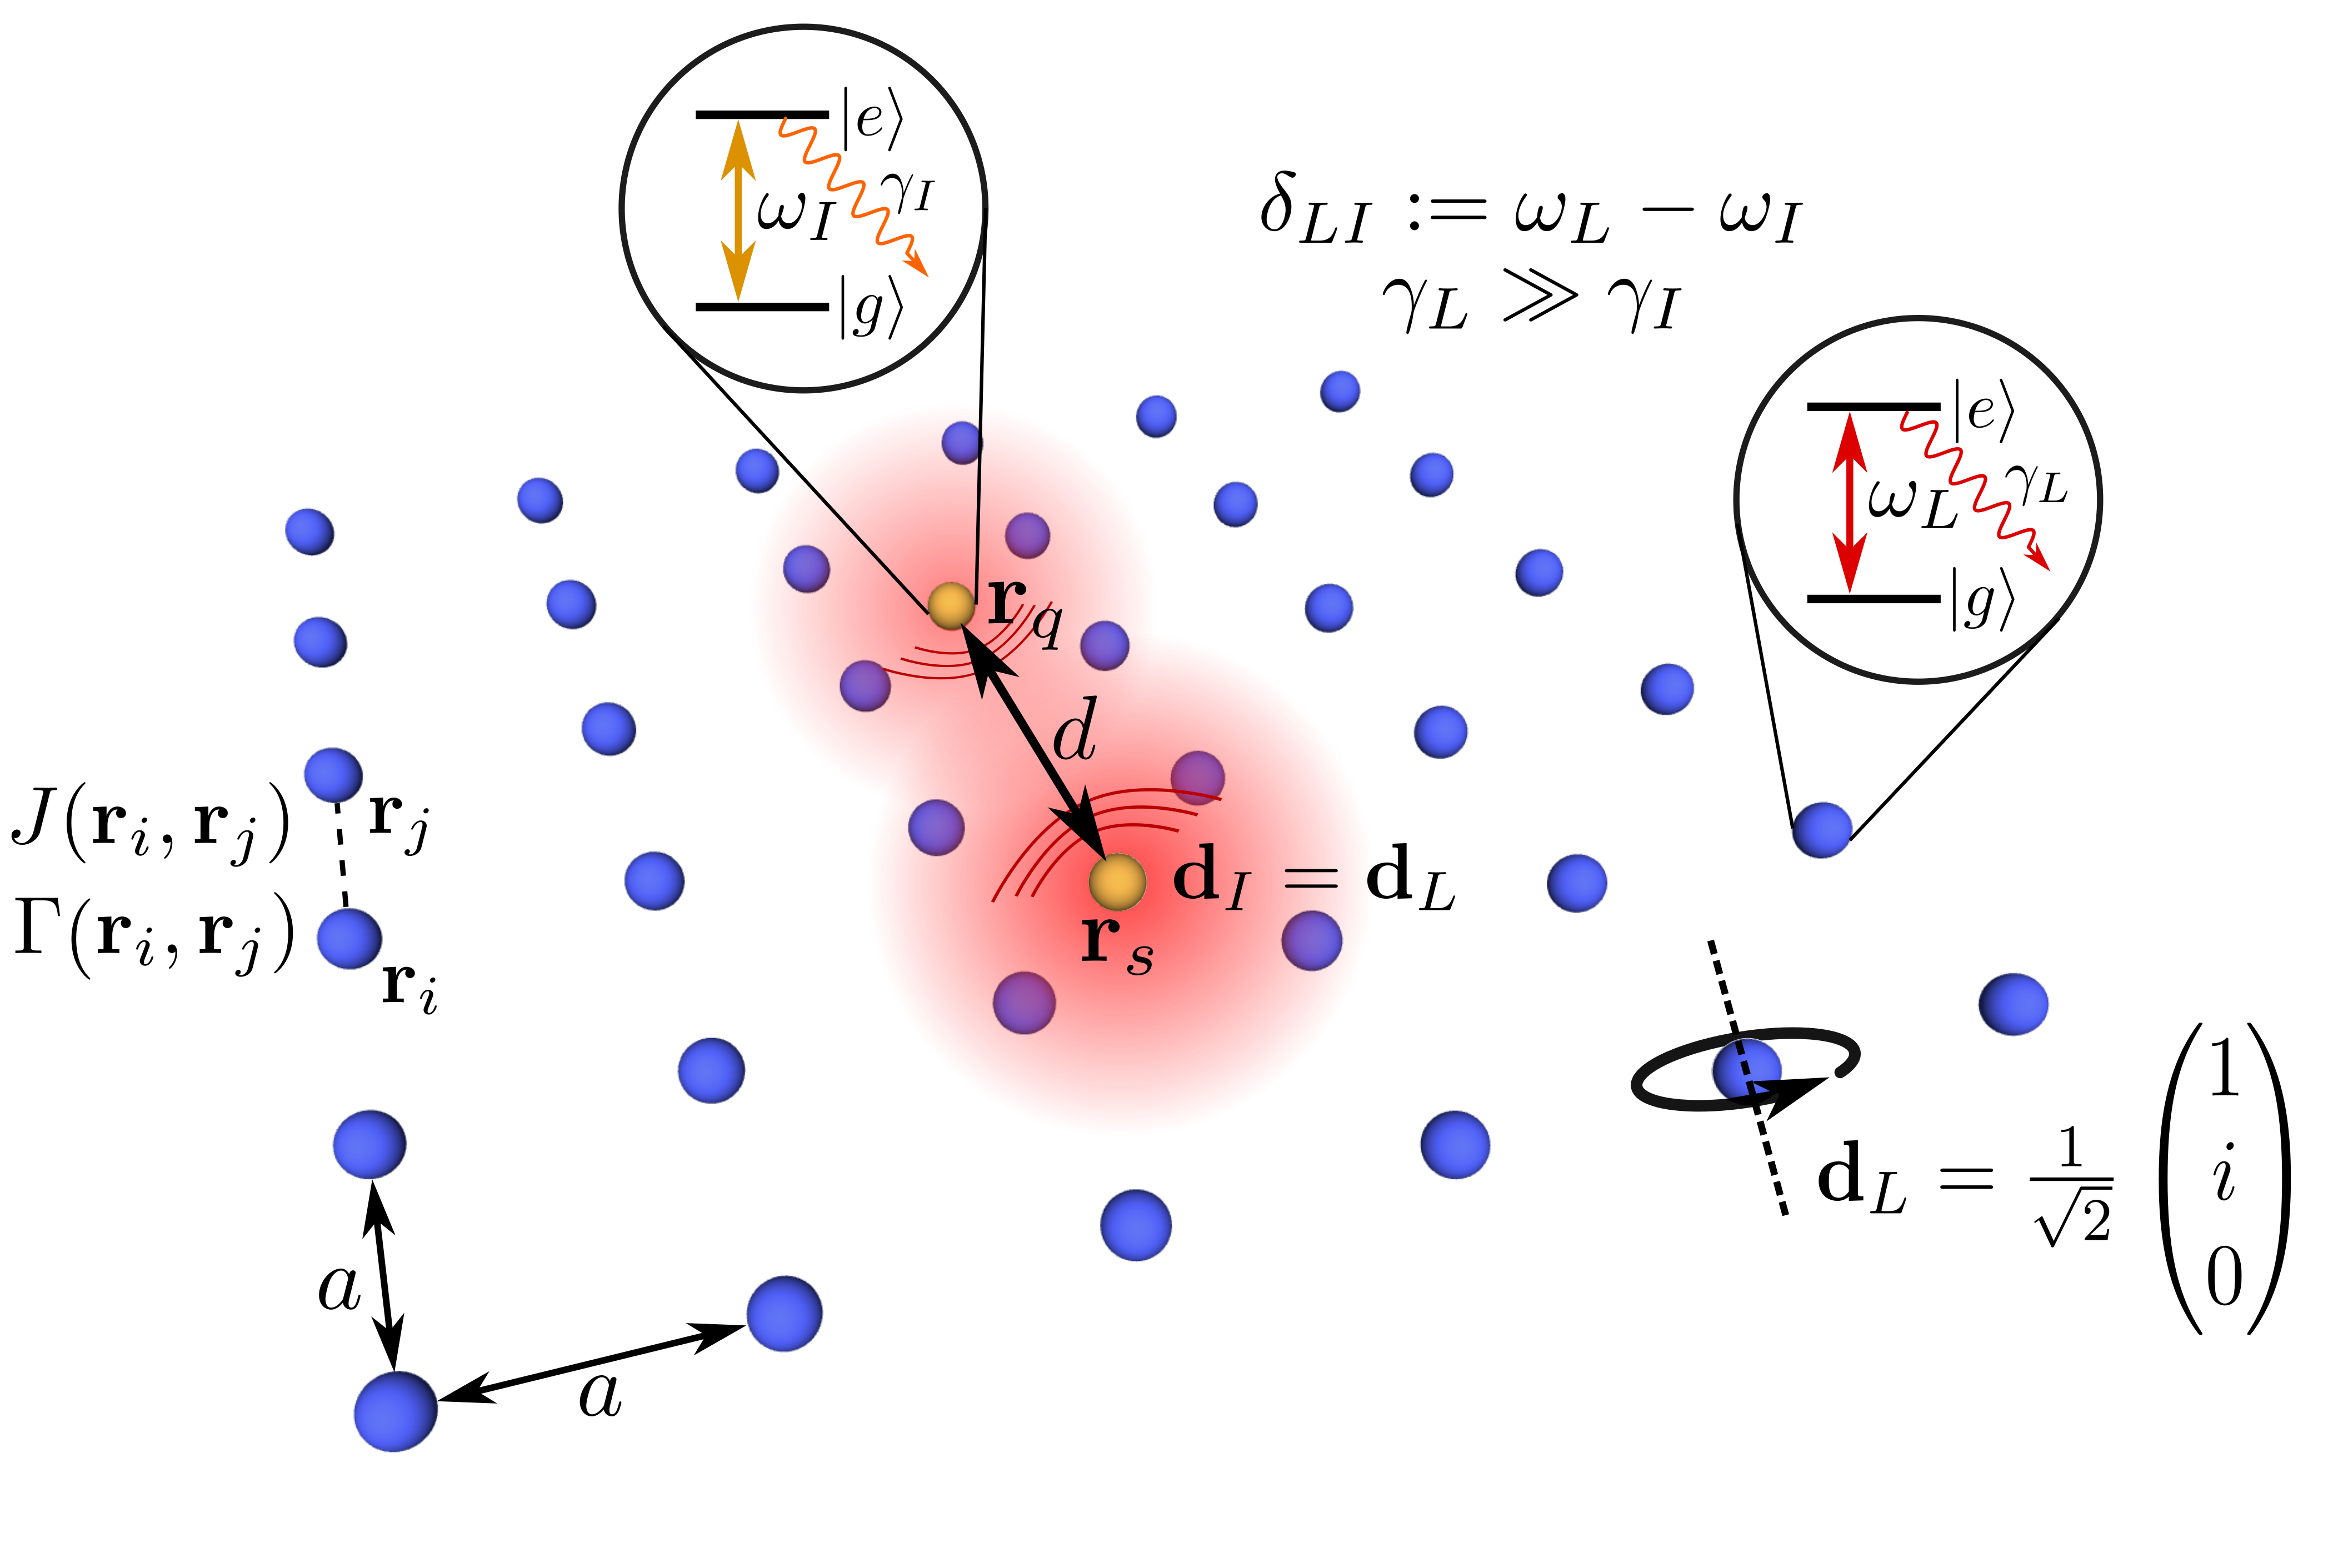
\includegraphics[width=0.4\textwidth]{figures/setup_2.png} 
\caption{•}
\label{fig:setup}
\end{figure}

% We see in~\eeref{eqn:Hamiltonian} and~\fref{fig:setup},~\eg test~\cite{kramer_quantumopticsjl_2018}

%==============================================================================================
\section{Model}
\commentSO{arb. geometry, Green's Tensor, Couplings, Polarizations -> Distance dependence, Hamiltonian, Self-energy, Ref. to Taylor's work}

We consider two-dimensional sub-wavelength lattices of quantum emitters which interact via resonant dipole-dipole interactions. The emitters are assumed to be two-level stems with a ground state $\ket{g}$ and an excited state $\ket{e}$ with a trasition frequency $\omega_L = c k_L$, such that $k_L = 2\pi/\lambda_L$ denotes the related wavenumber with the resonance wavelegth $\lambda_L$. Pairwise resonant dipole-dipole interactions among emitters result in collective couplings $J_{ij}$ and collective decay rates $\Gamma_{ij}$ between emitters $i$ and $j$ at positions $\rr_i$ and $\rr_j$, given by 
\begin{equation} J_{ij} = -\frac{3\pi \sqrt{\gamma_i \gamma_j}}{\omega_L} {\hat{d}^\dagger}_i \cdot \textbf{Re} [\textbf{G}(\textbf{r}_{ij}, \omega_L)] \cdot \hat{d}_j 
\label{eqn:J} \end{equation}
\begin{equation} \Gamma_{ij} = \frac{6\pi \sqrt{\gamma_i \gamma_j}}{\omega_L} {\hat{d}^\dagger}_i \cdot \textbf{Im} [\textbf{G}(\textbf{r}_{ij},\omega_L)] \cdot \hat{d}_j 
\label{eqn:Gamma} \end{equation}
where $\gamma_i$ and $\gamma_j$ are the decay rates of the individual dipoles $i$ and $j$, and $\rr_{ij} = \rr_i - r_j$ is the displacement vector. $\textbf{G}(\textbf{r}_{ij}, \omega_L)$ is the Green's tensor, defined as 

\begin{multline} 
    G_{\alpha\beta} (\textbf{r}, \omega) = \frac{e^{i\omega r}}{4\pi r} \left[ \left( 1 + \frac{i}{\omega r} - \frac{1}{\omega^2 r^2} \right) \delta_{\alpha\beta}
    \right. \\ \left. 
    - \left( 1 + \frac{3i}{\omega r} - \frac{3}{\omega^2 r^2} \right) \frac{r_\alpha r_\beta}{r^2} \right] - \frac{\delta(\textbf{r})}{3\omega^2} \delta_{\alpha\beta} 
    \label{eqn:Green}
\end{multline}

$d_i$ and $d_j$ are the dipole polarizations, which set to be uniformly circular, so that 

\begin{equation} 
    \hat{d}_L = \hat{d}_I = \frac{1}{\sqrt{2}} \begin{pmatrix}
    1 \\ i \\ 0
    \end{pmatrix} 
    \label{eqn:polarization}
\end{equation}

where $\hat{d}_L$ is the polarization of the lattice dipoles, and $\hat{d}_I$ is the polarization of any impurities. This polarization ensures that the dynamics of the system depend purely on the relative distances $r_{ij}$ between pairs of dipoles, independent of their relative orientations. As a result, $J_{ij}$ and $\Gamma_{ij}$ can be written as 
\begin{equation} J_{ij} = -\frac{3}{8 \omega_L r_{ij}} \left( \cos \omega_L r_{ij} + \frac{\sin \omega_L r_{ij}}{\omega_L r_{ij}} + \frac{\cos \omega_L r_{ij}}{(\omega_L r_{ij})^2} \right) \end{equation}
\begin{equation} \Gamma_{ij} = \frac{3}{4\omega_L r_{ij}} \left( \sin\omega_L r_{ij} - \frac{\cos\omega_L r_{ij}}{\omega_L r_{ij}} + \frac{\sin\omega_L r_{ij}}{(\omega_L r_{ij})^2} \right) \end{equation}

In this way, collective couplings (\fref{fig:J_r}) and collective decay rates (\fref{fig:Gamma_r}) depend purely on the relative distances $r_{ij}$ between pairs of dipoles, independent of their relative orientations. 
\begin{figure}
    % \centering
    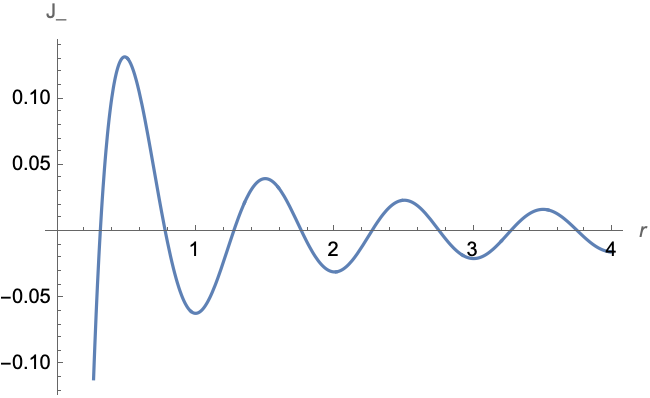
\includegraphics[width=0.4\textwidth]{figures/J(r).png} 
    \caption{•}
    \label{fig:J_r}
\end{figure}

\begin{figure}
    % \centering
    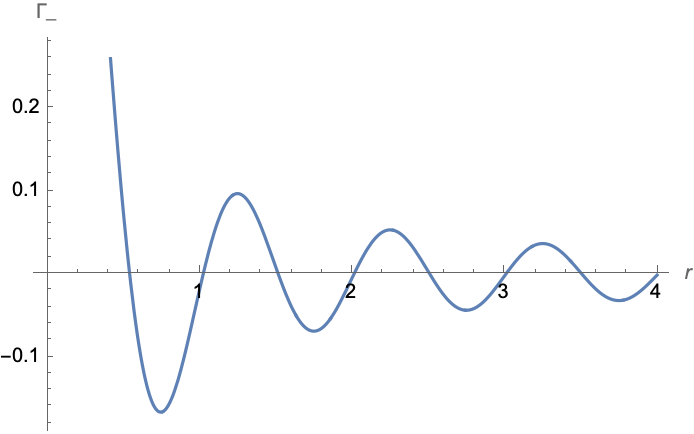
\includegraphics[width=0.4\textwidth]{figures/Gamma(r).png} 
    \caption{•}
    \label{fig:Gamma_r}
\end{figure}

\commentSB{It might be better if these figures go along with the first figure, at the top of this page}

Into this lattice, we place one or two lattice impurities with transition frequency $\omega_I \approx \omega_L$. The overall Hamiltonian is thus 

\begin{equation}   
    H = \sum_i^N \left( \omega_L - \frac{i}{2} \gamma_L \right) \sigma_i^\dag \sigma_i + \sum_{i,j \neq i}^N \left( J_{ij} - \frac{i}{2} \Gamma_{ij} \right) \sigma_i^\dag \sigma_j 
    \label{eqn:Hamiltonian}
\end{equation}

where $\sigma_i$ is the lowering operator of dipole $i$. 
\commentSB{Is this point about sigma necessary?}

\commentSB{Then, at some point here or later, explain the role of the detuning delta}

%==============================================================================================
\section{Single impurity case}
\commentSO{Define lattices, define distances related to lattices, $\Gamma_\mathrm{eff}$, constant area}

% \commentSB{Put the self-energy calculation here, along with the Gamma-eff calculation? Because I don't think there's anything more to say here. Any details about the geometries need to be left to the specific sections directly below here.}

The generic form of the Hamiltonian for a given lattice of $N$ atoms along with a single impurity is 

% \begin{equation}
%     H = \begin{pmatrix}
%         H_{11} & H_{12} & \cdots & H_{1N}  &  C_{LI,1}\\ 
%         H_{21} & H_{22} & & H_{2N}         & C_{LI,2} \\
%         \vdots & & \ddots & \vdots         & \vdots  \\
%         H_{N1} & H_{N2} & \cdots & H_{NN} & C_{LI,N} \\
%         C_{IL,1} & C_{IL,2} & \cdots & C_{IL,N} & H_I   
%     \end{pmatrix}
% \end{equation}
\begin{equation}
    H = \begin{pmatrix}
        ~ & ~ & ~ &   C_{LI} \\ 
        ~ & H_L & ~ & \vdots \\
        ~ & ~ & ~ & C_{LI} & \\
        C_{IL} & \cdots & C_{IL} & H_I   
    \end{pmatrix}
    \label{eqn:blockH1}
\end{equation}
where $H_L$ represents the $N \times N$ matrix of terms for the lattice's own Hamiltonian, $H_I$ is the lattice, and $C_{IL}$ along with $C_{LI}$ represent the coupling terms between the lattice atoms and the impurity. 
\commentSB{Firstly, is there some better notation than this, especially $C_{IL,1}$, with that comma there. Secondly, does $C_{IL,1} = C_{LI,1}$, or is there some other symmetry that can be exploited in the notation?}

Define the wavefunction such that
\begin{equation} \psi = 
\begin{pmatrix}
    b_1 \\ \vdots \\ b_N \\ c
\end{pmatrix} 
\label{eqn:psi}
\end{equation}
and assume that the lattice occupies a steady state, so that the Schr\"odinger equation is
\commentSB{This equation can maybe be eliminated, as it might be redundant. Is there a more appropriate phrasing than "steady state"?}

\begin{equation} i \hbar 
    \begin{pmatrix}
    0 \\ \vdots \\ 0 \\ \dot{c}
    \end{pmatrix} = \begin{pmatrix}
        ~ & ~ & ~ &   C_{LI} \\ 
        ~ & H_L & ~ & \vdots \\
        ~ & ~ & ~ & C_{LI} & \\
        C_{IL} & \cdots & C_{IL} & H_I   
    \end{pmatrix} \begin{pmatrix}
        b_1 \\ \vdots \\ b_N \\ c
    \end{pmatrix} 
\end{equation}
This can be solved to get 
\begin{equation}
    \begin{pmatrix}
        b_1 \\ \vdots \\ b_N
    \end{pmatrix} = - H_L^{-1} C_{LI} c
\end{equation}
Putting this back into the Schr\"odinger equation produces 
\begin{equation}
    \dot{c} = -i (H_I - C_{IL}^T H_L^{-1}C_{LI}) c
\end{equation}
Recognizing that $ H_I - C_{IL}^T (H_L^{-1}) C_{LI} = \Sigma_I - i \frac{\gamma_I}{2} $, we can calculate the impurity's self-energy $\Sigma_I$ to be 
\commentSB{Should this identification be justified?}
\begin{equation}
    \Sigma_I = H_I - C_{IL}^T (H_L^{-1}) C_{LI} + i \frac{\gamma_I}{2}
    \label{eqn:selfenergy}
\end{equation}
The effective decay rate $\Gamma_\text{eff}$ for an impurity in the lattice is related to this self-energy according to 
\begin{equation}
    \Gamma_\text{eff} = \gamma_I - 2~\im[\Sigma_I]
\end{equation}
% \begin{equation}
%     H = 
%     \begin{pmatrix}
%         -\frac{i \gamma_L}{2} - \frac{\delta_{LI}}{2} & J(r_{12}) - \frac{i \Gamma(r_{12})}{2} & \cdots \\
%         J(r_{21}) - \frac{i \Gamma(r_{21})}{2} & -\frac{i \gamma_L}{2} - \frac{\delta_{LI}}{2} & & \\
%         \vdots & & \ddots

%     \end{pmatrix}
% \end{equation} 


% \commentTP{Draw a diagram of the four parts of the Hamiltonian to set up the self-energy calculation.}



In order to reasonably compare lattices of differing geometries, we ensure whenever possible that all plaquettes possess the same area.
% , because...
% \commentSB{Does this argument rely on a momentum-space view of things? In any case, make this constant area argument rigorous}

------------------------

\commentSB{This is just a holding space for this matrix, in case we want to copy and paste it to anywhere. I don't actually intend for it to sit here in this section.}

\begin{equation}
    H = 
    \begin{pmatrix}
        -\frac{i \gamma_L}{2} - \frac{\delta_{LI}}{2} & J(r_{12}) - \frac{i \Gamma(r_{12})}{2} & \cdots \\
        J(r_{21}) - \frac{i \Gamma(r_{21})}{2} & -\frac{i \gamma_L}{2} - \frac{\delta_{LI}}{2} & & \\
        \vdots & & \ddots
    \end{pmatrix}
\end{equation}


\subsection{Square vs. triangular}

Consider a finite square lattice, with an inter-atomic spacing of $a = 0.2$, defined as a function of \commentSB{that characteristic wavelength}. 

Compare this to a triangular lattice with the same inter-atomic spacing. 
\commentSB{see earlier point about how we should really use constant area}

\commentTP{Put a figure that just shows a single plaquette for each of our two cases here, with dots going off in 4 and 3 directions respectively}

%=================
\subsubsection{Interstitial}
\commentSO{Interstitial which imposes one more length scale -> refer to analytics, numerics -> impurity position}
Now, consider an impurity atom placed within a plaquette. For the square case, we implemented this arrangement using a $4\times 4$ lattice, so that the impurity was centered within the lattice. 

\commentSB{Put a small diagram here? You can illustrate the length scales here as well}

Likewise, for the triangular case, we placed the impurity at the center of a \commentSB{12 atom?} lattice, with the following arrangement. 

\commentSB{diagram?}

By placing the impurity at the center of a plaquette, only one additional length scale is introduced. 
%  Hence, the coupling as a function of inter-atomic spacing is \commentSB{fairly constant, looking at the analytics?} 

% \commentSB{J and Gamma diagrams}

% \commentSB{Should we vary inter-atomic spacing?}

After attempting to place the impurity off-center, 

\commentTP{Have a plot of Gamma over delta, to justify how we choose an "optimum" delta}

\commentSB{numerics plaquette plots}

it is clear that the point at which the impurity atom experiences minimal decay is at the center of the plaquette. 

\commentSB{plaquette lineplots showing minimal Gamma}

This point also possesses the highest symmetry, suggesting that additional symmetries lead to slower decay rates. This hypothesis is supported by the behavior of the coupling constants for various positions of the impurity away from the center 

\commentSB{a diagram of this description, which has not been made yet. Or perhaps two diagrams, one moving from the center to a lattice point, and another moving from the center to the midpoint between two lattice points. Actually, four diagrams, because these two should be made for both the square and triangular cases}


%=================
\subsubsection{Substitution}
\commentSO{Does NOT(!) impose another length scale as long as it is not away from the center -> refer to analytics, -> always at band edge, numerics -> impurity position}

Now, considering substituting a lattice atom for an impurity, so that, in effect, the impurity takes up a vacancy in the lattice. For the square lattice, we used this $5 \times 5$ geometry for our analysis:

\commentSB{diagram}

and for the triangular lattice, we used this geometry

\commentSB{probably an 18 atom lattice?}

Performing this substitution on the lattice introduces no additional length scales, as long as the impurity is placed at the center of the vacancy. If it is placed off-center, the best possible values of $\Gamma_\text{eff}$ are 

\commentSB{plaquette plots from numerics}

Once again, the point with the highest symmetry experience  minimal decay rates

\commentSB{plaquette lineplots showing minimal Gamma}

\commentSB{Maybe include another analytic plot showing how symmetry changes coupling constants? Just do this for square lattice.}

%==============================================================================================
\subsection{Monoclinic vs. rectangular lattice}
\commentSO{similar arguments}

Now, consider the Bravais lattices defined by variable paramters. 

In particular, consider a monoclinic lattice defined by $\theta$, such that at $\theta = \frac{\pi}{2}$ we recover the square lattice case with an inter-atomic spacing of $0.2$. By maintaining a constant vertical distance between the layers of the lattice, we ensure that the area of the plaquettes remains constant over the range $ 0 < \theta \leq \frac{\pi}{2}$. 

\commentSB{diagram of this geometry}

%=================
\subsubsection{Interstitial}


%=================
\subsubsection{Substitution}

%=================
\subsubsection{Varying scaling factors}
\commentSO{justify why we use interstitial in the following}

%==============================================================================================
\section{Two impurity case}
\commentSO{Q-factor, analyze different lattices -> discuss the most important figures, constant distance}

$\Gamma_\text{eff}$ for a lattice with two impurities is calculated in a manner analagous to the single-impurity case, starting with the Schr\"odinger equation for the two-impurity Hamiltonian, for which  
\commentSB{Perhaps write out the meanings of all these new variables, if it's not clear}
\begin{equation}
    i \hbar \begin{pmatrix}
        0 \\ \vdots \\ 0 \\ \dot{c} \\ \dot{d}
    \end{pmatrix}
    = \begin{pmatrix}
        ~ & ~ & ~ &   C_{L1} & C_{L2} \\ 
        ~ & H_L & ~ & \vdots & \vdots \\
        ~ & ~ & ~ & C_{L1} &  C_{L2} \\
        C_{1L} & \cdots & C_{1L} & H_1 & C_{12} \\
        C_{2L} & \cdots & C_{2L} & C_{21} & H_2  
    \end{pmatrix} 
    \begin{pmatrix}
        b_1 \\ \vdots \\ b_N \\ c \\ d
    \end{pmatrix}
    \label{eqn:blockH2}
\end{equation}
In this way, 
\begin{equation}
    b = -(H_L)^{-1} (C_{L1} c + C_{L2} d)
\end{equation}
Putting this result back into the Schr\"odinger equation gives 
\begin{equation}
    \dot{c} = -i \left[  H_1 - {C_{1L}}^T (H_L)^{-1} C_{L1}\right] c - i \left[  C_{12} - {C_{1L}}^T (H_L)^{-1} C_{L2} \right] d
\end{equation}
\begin{equation}
    \dot{d} = -i \left[  H_2 - {C_{2L}}^T (H_L)^{-1} C_{L2}\right] c - i \left[  C_{21} - {C_{2L}}^T (H_L)^{-1} C_{L1} \right] d 
\end{equation}
Let $\dot{c} = -i [\Sigma_1 - \frac{i \gamma_1}{2}]c - i \kappa_1 d $ and $\dot{d} = -i [ \Sigma_2 - \frac{i \gamma_2}{2} ] d - i \kappa_2 c $, where $\kappa_1$ and $\kappa_2$ are ``effective couplings.'' Solving for these and the self-energies results in 
\begin{equation}
    \Sigma_1 = H_1 - {C_{1L}}^T (H_L)^{-1} C_{L1} + \frac{i \gamma_1}{2}
\end{equation}
\begin{equation}
    \Sigma_2 = H_2 - {C_{2L}}^T (H_L)^{-1} C_{L2} + \frac{i \gamma_2}{2}
\end{equation}
\begin{equation}
    \kappa_1 = C_{12} - {C_{1L}}^T (H_L)^{-1} C_{L2} 
\end{equation}
\begin{equation}
    \kappa_2 = C_{21} - {C_{2L}}^T (H_L)^{-1} C_{L1} 
\end{equation}
\commentSB{As a general point: At some point, take note of which equation to give numbers and which to not. Because right now, I'm just reflexively giving them all numbers for simplicity's sake.}
The impurities' effective decay rates are 
\begin{align}
    \Gamma_\text{eff,1} = \gamma_1 - 2~\im[\Sigma_1] &&
    \Gamma_\text{eff,2} = \gamma_2 - 2~\im[\Sigma_2]
\end{align}
We define the Q-factor as a function of the effective decay rate and the effective coupling, so that 
\begin{align}
    Q_1 = \frac{re[\kappa_1]}{\Gamma_\text{eff,1}} && Q_2 = \frac{re[\kappa_2]}{\Gamma_\text{eff,2}} 
\end{align}

%=================
\subsection{Monoclinic lattice}


%=================
\subsection{Rectangular lattice}


%==============================================================================================
\section{Conclusions and Outlook}\label{sec:conclusion}

These are the Conclusions.\\[2ex]

\emph{Acknowledgments.} We would like to thank \commentSO{add people}. This work was supported by \commentSO{add funding sources}

The numerical simulations were performed with the open-source framework \texttt{QuantumOptics.jl}~\cite{kramer_quantumopticsjl_2018}.


\bibliographystyle{apsrev4-1-title}
\bibliography{references_optimized_geometries}

\end{document}

